
\documentclass[tikz, border=5mm]{standalone}
% \pagecolor{transparent}
\usepackage{tikz}
\usepackage{xstring}
\usetikzlibrary{decorations.pathreplacing}
\usetikzlibrary{math, calc, shapes.misc, shapes}
\begin{document}
  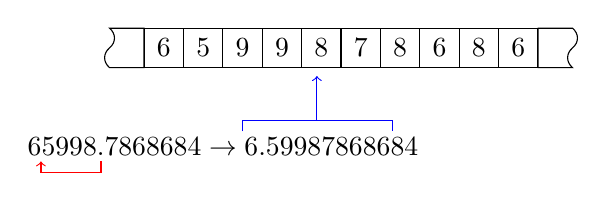
\begin{tikzpicture}[digits/.style={inner xsep=0pt, inner ysep=2pt}]
        \node[digits] (one) at (0,0) {$65998.7868684 \rightarrow 6.59987868684$};
              \draw[<-, red] ([xshift={width("$6$")}]one.south west) to ([xshift={width("$6$")}, yshift=-4]one.south west) to ([xshift={width("$65998.$")-0.5ex/2}, yshift=-4]one.south west) to ([xshift={width("$65998.$")-0.5ex/2}]one.south west);
        \draw[fill=none](-1, 1) rectangle ++(0.5,0.5) node[pos=0.5]{$6$};
        \draw[fill=none](-0.5, 1) rectangle ++(0.5,0.5) node[pos=0.5]{$5$};
        \draw[fill=none](0, 1) rectangle ++(0.5,0.5) node[pos=0.5]{$9$};
        \draw[fill=none](0.5, 1) rectangle ++(0.5,0.5) node[pos=0.5]{$9$};
        \draw[fill=none](1, 1) rectangle ++(0.5,0.5) node[pos=0.5]{$8$};
        \draw[fill=none](1.5, 1) rectangle ++(0.5,0.5) node[pos=0.5]{$7$};
        \draw[fill=none](2, 1) rectangle ++(0.5,0.5) node[pos=0.5]{$8$};
        \draw[fill=none](2.5, 1) rectangle ++(0.5,0.5) node[pos=0.5]{$6$};
        \draw[fill=none](3, 1) rectangle ++(0.5,0.5) node[pos=0.5]{$8$};
        \draw[fill=none](3.5, 1) rectangle ++(0.5,0.5) node[pos=0.5]{$6$};
        \node[tape, rotate=-90,draw, tape bend top=none,tape bend height=0.125cm,
            tape bend bottom=out and in,fill=none, minimum width=0.5cm,minimum height=0.5cm] at (-1.19, 1.25) {};
        \node[tape, rotate=90,draw, tape bend top=none,tape bend height=0.125cm,
            tape bend bottom=out and in,fill=none, minimum width=0.5cm,minimum height=0.5cm] at (4.19, 1.25) {};
\draw[-, blue] ([xshift={width("$65998.7868684 \rightarrow 6$")-1.25ex}]one.north west) to ([xshift={width("$65998.7868684 \rightarrow 6$")-1.25ex}, yshift=4]one.north west) to ([xshift={width("$65998.7868684 \rightarrow 6.599878686$")+0.5ex/2}, yshift=4]one.north west) to ([xshift={width("$65998.7868684 \rightarrow 6.599878686$")+0.5ex/2}]one.north west);
\draw[->, blue] ([xshift={width("$65998.7868684 \rightarrow 6$")+width("$6.5998786$")/2},yshift=4]one.north west) to ([xshift={width("$65998.7868684 \rightarrow 6$")+width("$6.5998786$")/2}, yshift=20]one.north west);
  \end{tikzpicture}
\end{document}
